\subsection{HTTP}
\label{sec:http}

Beim \ac{http} handelt es sich um ein zustandsloses Protokoll zur Datenübertragung, dessen Haupteinsatzgebiet im Internet ist. Über \ac{http} werden Web-Ressourcen von einem Server zu einem Webbrowser übertragen. Hierbei kommunizieren der Webserver und der Webbrowser über das Protokoll. Der Ablauf erfolgt in etwa wie in \autoref{img:http-simple}.

\begin{figure}[H]
	\begin{center}
		\includegraphics[width=0.5\textwidth]{http-simple.png}
		\caption{Kommunikationsbeispiel mit HTTP}
		\label{img:http-simple}
	\end{center}
\end{figure}

%\begin{figure}[htbp]
%	\centering
%	\includesvg{http-simple}
%	\caption{svg image}
%\end{figure}

Der Client fordert vom Server, dem der Hostname www.example.com zugewiesen ist, die gewünschte Web-Ressource, hier index.html, an. Zusätzlich wird die gewünschte HTTP-Methode, hier GET, und die HTTP-Version, hier 1.1, definiert. Weiterhin ist das Versenden weiterer Parameter möglich. Diese Anfrage wird auch HTTP-Request genannt. Anschließend antwortet der Server im Erfolgsfall mit der angeforderten Ressource und weiteren Metainformation, im Fehlerfall mit einem entsprechenden Statuscode. Die Antwort des Servers nennt sich HTTP-Response.\\
Im Normalfall besteht eine Webseite aber nicht nur aus einer HTML-Seite, sondern noch aus weiteren Ressourcen. Diese werden, zumindest in der HTML-Version 1.1, in etwa wie in \autoref{img:http} übertragen. Zu beachten ist, dass diese und folgenden Abbildungen im Gegensatz zur \autoref{img:http-simple} vereinfacht wurden und bewusst auf Informationen wie die HTTP-Methode und die HTTP-Version verzichtet wird.

\begin{figure}[H]
	\begin{center}
		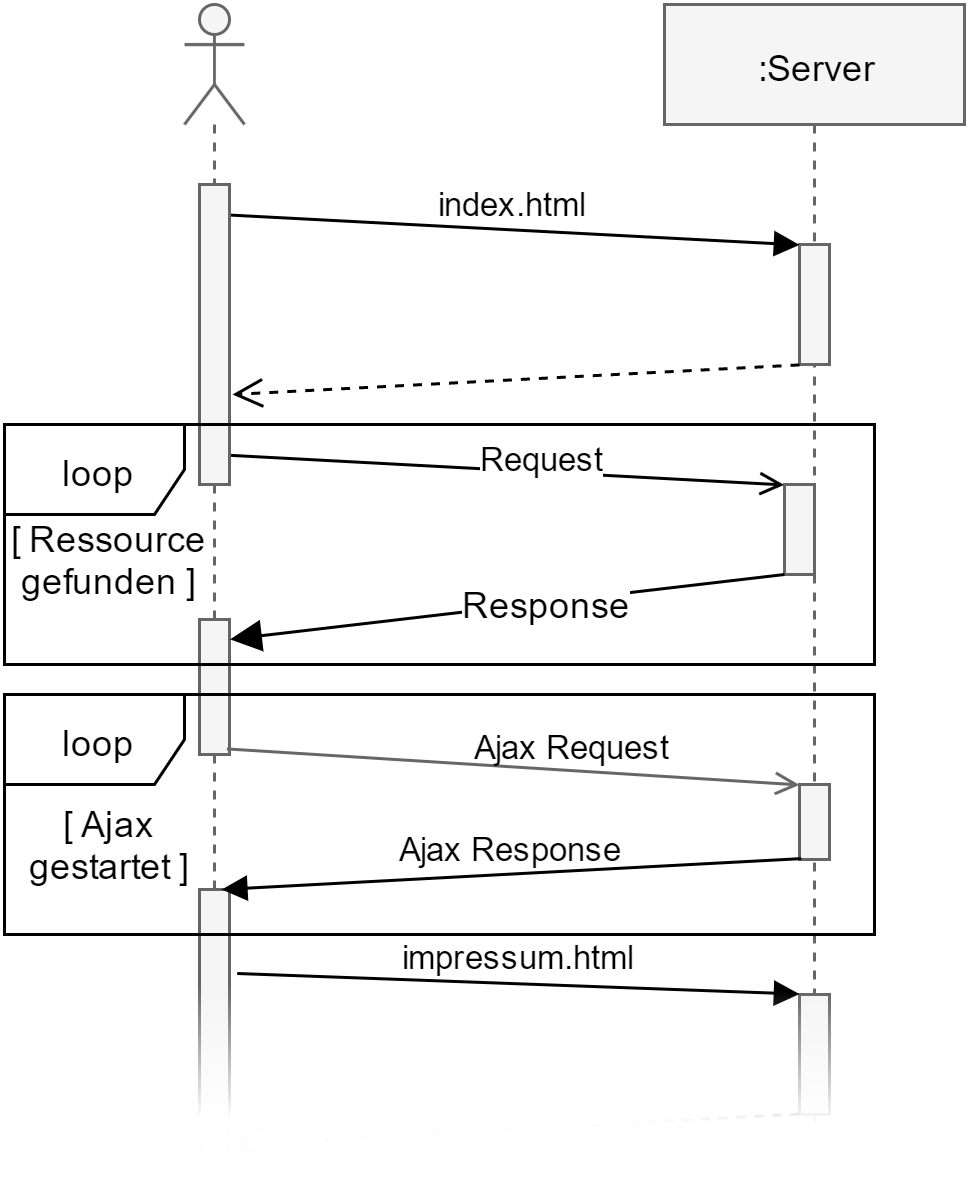
\includegraphics[width=0.5\textwidth]{http.png}
		\caption{Ladevorgang einer Webseite}
		\label{img:http}
	\end{center}
\end{figure}

Zunächst wird die eigentliche Webseite, am Beispiel \autoref{img:http} wäre dies index.html, angefordert. Nachdem diese vollständig geladen ist, durchsucht der Webbrowser den erhaltenen Quellcode nach weiteren Web-Ressourcen, wie Grafiken, Skripte, Stylesheets etc. und fordert auch diese vom Webserver an. Dabei können mehrere Anfragen gleichzeitig ausgeführt werden. Der Webbrowser achtet aber darauf, dass unter anderem Skripte in der gleichen Reihenfolge ausgeführt werden, wie diese im Quellcode der Webseite auftauchen, auch wenn ein später auftauchendes kleines Skript früher vollständig geladen wurde als eine zuvor erscheiende Bibliothek, um Abhängigkeitsfehler zu vermeiden. Weitere Web-Ressourcen kann der Client nun über Ajax anfordern, siehe hierzu \autoref{sec:ajax}. \\
Möchte der Benutzer nun die Seite wechseln, zum Beispiel nach impressum.html, würde sich der Prozess entsprechend, gegebenenfalls mit anderen Ressourcen, wiederholen. \\

Einfach ausgedrückt, wird eine Webseite also wie folgt geladen.

\begin{description}
	\item[HTML-Seite:] Die darzustellende HTML-Seite wird vom Server angefordert.
	\item[Web-Ressourcen:] Der Quellcode der HTML-Seite wird nach weiteren Web-Ressourcen, wie Grafiken, Skripte oder Stylesheets, durchsucht und diese werden geladen.
	\item[Ajax:] Ajax Anfragen werden ausgeführt.
\end{description}